\documentclass[12pt]{beamer}
\usepackage[utf8]{inputenc}
\usepackage[T2A, T1]{fontenc}
\usepackage[british, french, russian]{babel}
\usepackage[style=ieee]{biblatex}
\usepackage[most]{tcolorbox}
\usepackage{graphicx}
% \usepackage{animate}
\usepackage{xurl}
\usepackage{setspace}
\usepackage{ragged2e}
\usepackage{indentfirst}
\usepackage{mathptmx}
\usepackage{pdfpages}
\usepackage{geometry}
\usepackage{amsmath}
\usepackage{amssymb}
\usepackage{txfonts}
\usepackage{multicol}
\usepackage{fancyhdr}
\usepackage{wrapfig}
\usepackage{array}
\usepackage{float}
\usepackage{alltt}
\usepackage{tabularx}
\usepackage{caption}
\usepackage{fancyvrb}
\usepackage{fvextra}
\usepackage{enumitem}
\usepackage{bigfoot}
\usepackage{hyperref}
\hypersetup{
    colorlinks = true,
    linkcolor = blue,
    urlcolor = blue,
    filecolor = blue,
    citecolor = blue
}
\usetheme{CambridgeUS}
\usecolortheme{spruce}
\author{F. Elion Galiba, K. Noché \&{} R. Sivathasan}
\title{\textbf{MU4RBI01 --~Projet \emph{Python}}}
\subtitle{\emph{Draconic Generations}}
\institute{Sorbonne Université}
\logo{
\includegraphics[width=0.125\textwidth]{SdI.png}}
\date{\today}
\beamertemplatenavigationsymbolsempty


\begin{document}
    \selectlanguage{french}
    \maketitle

    % =====
    % Ramya
    % =====

    \section{\emph{Draconic Generations}} % Présentation du jeu et essai du jeu.
        \begin{frame} % Teste du jeu à cette slide.
            \frametitle{Le Jeu}
            \begin{figure}[H]
                \centering
                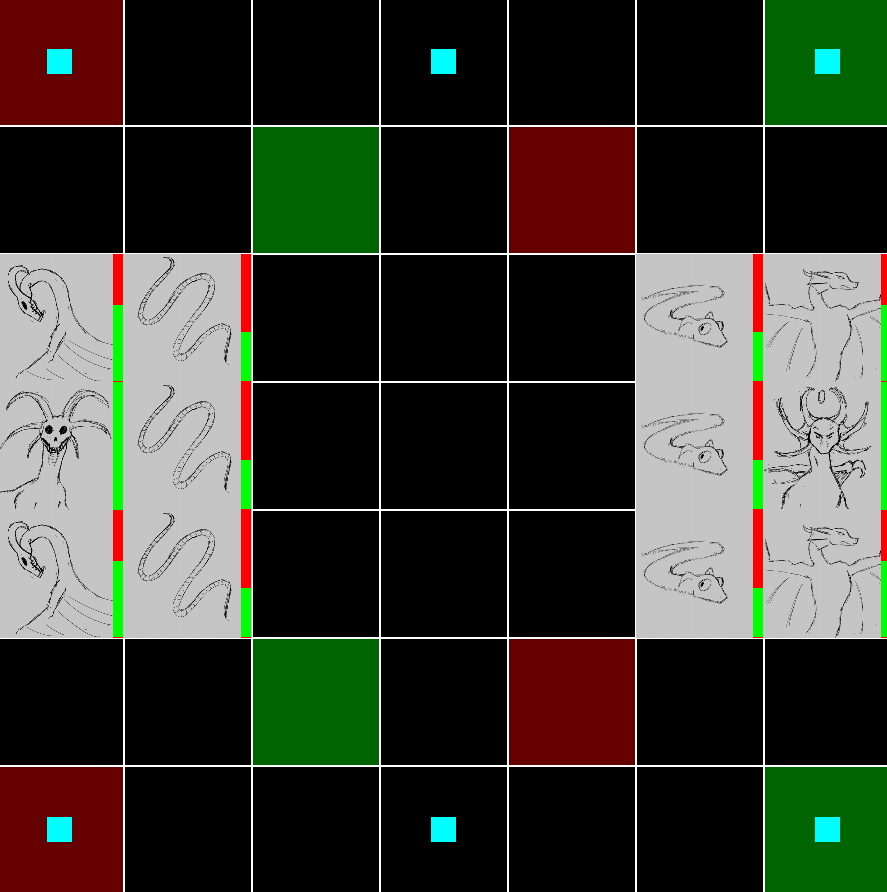
\includegraphics[width=0.6\textwidth]{ImageDuJeu.png}
            \end{figure}
        \end{frame}

    % =====
    % Kévin
    % =====

    \section{Le Code} % Présentation du code.
        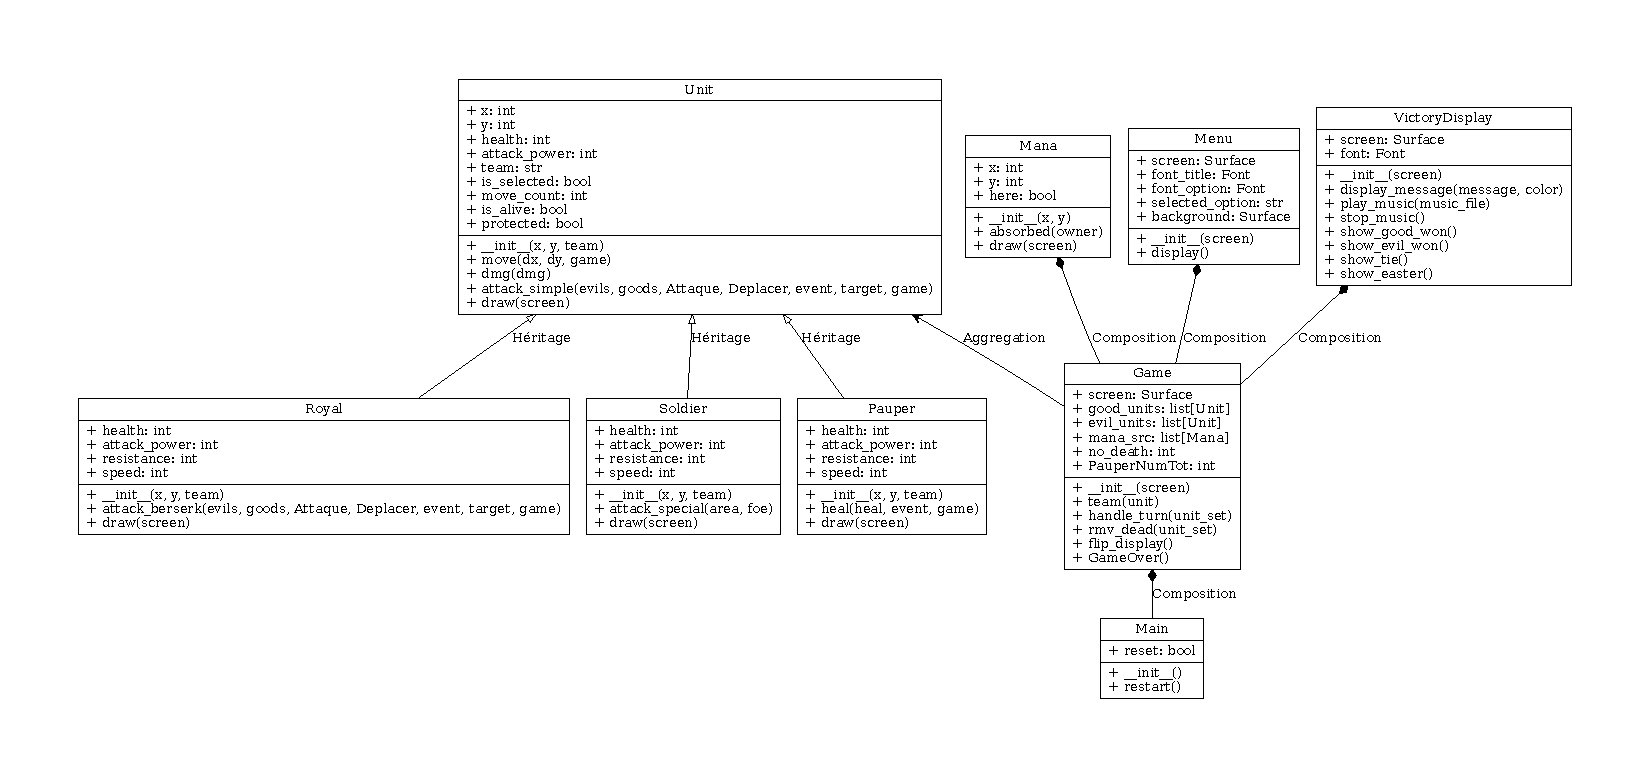
\includepdf{UML.pdf}
        \begin{frame}[fragile]
            \frametitle{\emph{Main}}\centering
            \pause
            \texttt{\_\_init\_\_()} = \texttt{main()}
            \pause
            \begin{block}{Comment recommencer?}
                \begin{verbatim}
    def restart(self):
        self.__init__()
                \end{verbatim}
            \end{block}
        \end{frame}
        \begin{frame}
            \frametitle{\emph{Game}}\centering
            \pause
            \texttt{handle\_turn()}\\
            \pause
            \texttt{rmv\_dead()}\\
            \pause
            \texttt{GameOver()}
        \end{frame}

        % =====
        % Ramya
        % =====

        \begin{frame}
            \frametitle{\emph{Unit}}\centering
            \pause
            \begin{itemize}
                \item{$\rightarrow$} Définition des \underline{fonctions communes}
                \pause
                \item{$\rightarrow$} \underline{Abstraite} et héritage avec autres unités
            \end{itemize}
        \end{frame}

        % ====
        % Fady
        % ====

        \begin{frame}
            \frametitle{\emph{VictoryDisplay}}\centering
            \pause
            \begin{itemize}
                \item{$\rightarrow$} Possibilité de recommencer
                \pause
                \item{$\rightarrow$} 1 fonction = 1 fin de partie % Il s'agit de show_evil_won(), show_tie(), etc...
            \end{itemize}
        \end{frame}
        \begin{frame}
            \frametitle{\emph{Menu}}\centering % Parler aussi de la gestion d'erreur?
            \pause
            Affichage de début\\
            +~Gestion de 2 boutons \&{} musique
        \end{frame}

    \section{Conclusion} % Conclusion.
        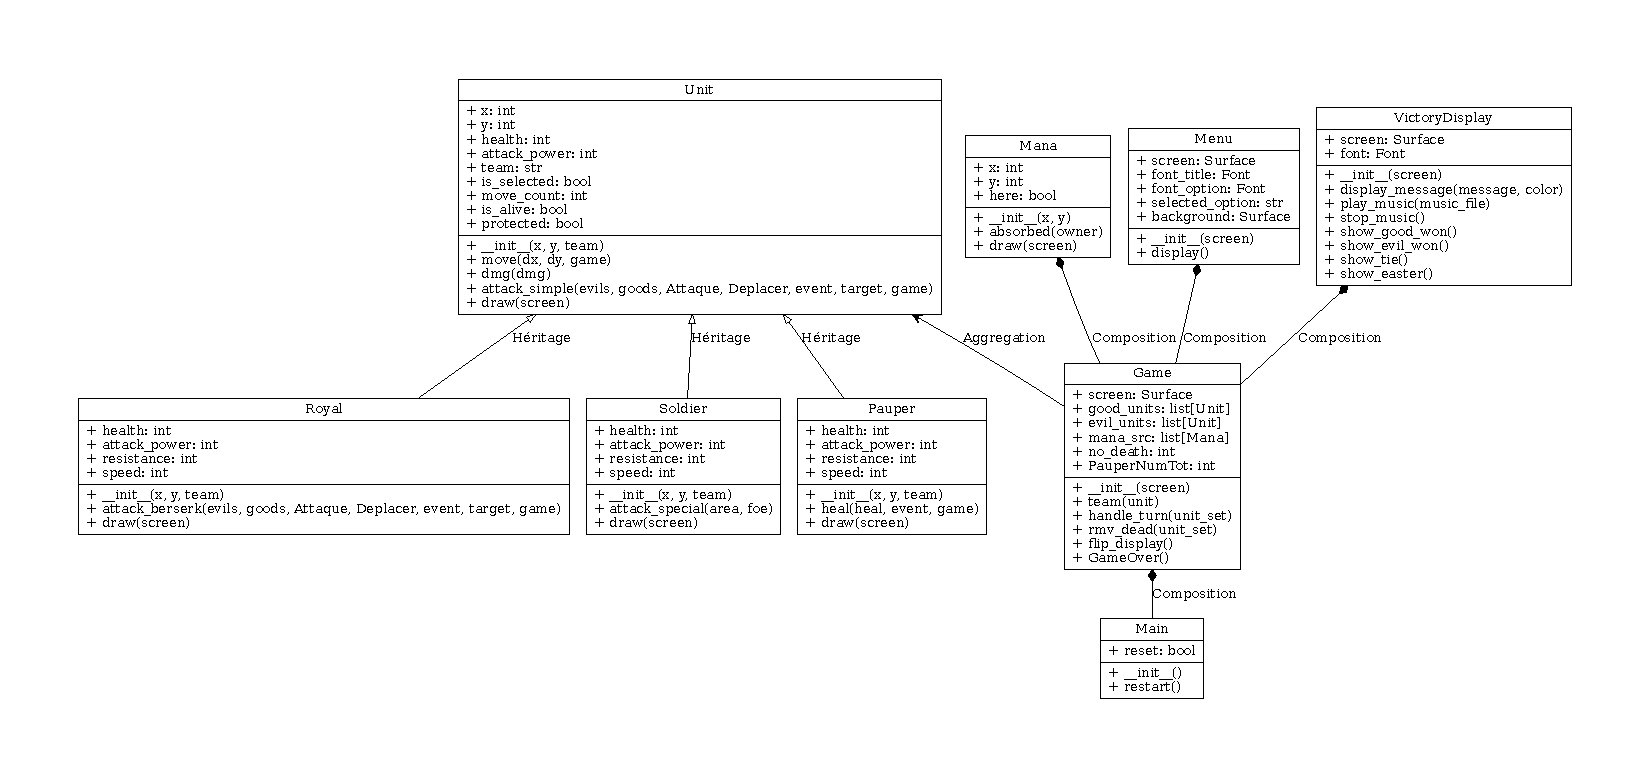
\includepdf{UML.pdf}
        \begin{frame}\thispagestyle{empty}\centering
            \Huge
            \textbf{MERCI POUR VOTRE ATTENTION!}
        \end{frame}
\end{document}
